\documentclass[a4paper]{article}

\usepackage[T1]{fontenc}
%\usepackage[utf8]{inputenc}
\usepackage[italian]{babel}
\usepackage{amssymb}
\usepackage{hyperref}
\usepackage{mathtools}
\usepackage{amsthm}
\usepackage[ruled,vlined,noend]{algorithm2e}

%%%%%%%%%%%%%%%%%%%%%%%%%%%%%%%%%%%%
\usepackage{listings} 
\lstdefinestyle{mystyle}{
    breakatwhitespace=false,                   
    captionpos=b,                    
    keepspaces=true,                 
    numbers=left,                    
    numbersep=5pt,                  
    showspaces=false,                
    showstringspaces=false,
    showtabs=False,                  
    tabsize=2
}

\lstset{style=mystyle}

\usepackage{setspace}
\singlespacing
%%%%%%%%%%%%%%%%%%%%%%%%%%%%%%%%%%%%
\usepackage{ulem} 
\usepackage{soul}

\usepackage{graphicx}
\graphicspath{ {./images/} }
%%%%%%%%%%%%%%%%%%%%%%%%%%%%%%%%%%%%

\mathtoolsset{showonlyrefs}  
\hypersetup{
    colorlinks=true,
    linkcolor=black,
    filecolor=black,      
    urlcolor=black,
}

\newcommand{\pluseq}{\mathrel{{+}{=}}}

\newtheorem {theorem}{Theorem}
\newtheorem{corollary}{Corollary}
\newtheorem{lemma}{Lemma}
\newtheorem{remark}{Remark}
\newtheorem{definition}{Definition}

\setcounter{secnumdepth}{3}
\setcounter{tocdepth}{3}

\title{Architectures for Big Data}
\author{Federico Bruzzone}
%\date{}
\makeindex

\begin{document}
\maketitle
\newpage
% \setlength{\parskip}{0.15em}
\tableofcontents
\setlength{\parindent}{0pt}
\setlength{\parskip}{0.8em}
\newpage

%\section{section}
...

\subsection{subsection}
	
\paragraph{paragraph}

\begin{remark}
    ...
\end{remark}

\subsubsection{subsubsection}

\subsubsection{subsubsection}

\paragraph{paragraph}

\subsection{subsection}
...
\begin{enumerate}
    \item 
    \item
    \item 
\end{enumerate}

\begin{itemize}
	\item 
    \item 
\end{itemize}

\begin{theorem}
    $PO \subseteq NPO$
\end{theorem}
\begin{proof}
    ...
\end{proof}

\begin{equation}
    \begin{aligned}
        \mathit{APX} = \{\Pi | \Pi \mathit{\;di\;ottimizzazione\;t.c.\;}
\exists \rho \geq 1, A, \\\mathit{t.c\;} x\rightarrow A \rightarrow y(x)\;\mathit{con}\;R_\Pi(x, y) \leq \rho\}
    \end{aligned}
\end{equation}


\paragraph{Algoritmo di risoluzione}
L'algoritmo di risoluzione è abbastanza semplice e si basa sulla 
ricerca di un cammino aumentante.

\begin{algorithm}[H]
    \SetAlgoLined
    \KwIn{$G=(V,E)$}
    \KwResult{Matching $M$ per $G$}
     $M \gets \emptyset$\\
     \While{$\Pi = \mathit{findAugmenting(G)}$}{
        $M.update(\Pi)$
     }
     \Return{M}
     \caption{BiMaxMatching}
\end{algorithm}


\subsection{Tecniche greedy}
Nella sezione a seguire si presentano problemi di ottimizzazione per cui 
tecniche greedy funzionano abbastanza bene. 
I problemi affrontati sono quelli di \emph{Load Balancing}, \emph{Center Selection} e \emph{Set Cover}.

\subsubsection{Load balancing}
\label{lb}
Il problema di Load Balancing può essere visto come il compito
di assegnare a macchine dei lavori da compiere, che richiedono del tempo, 
in modo da minimizzare il tempo totale.


\begin{theorem}
    Load Balancing è NPO completo
\end{theorem}
Bisogna perciò trovare un modo di approssimare una soluzione.
\paragraph{Greedy balance}
Il primo approccio alla risoluzione del problema è quello di assegnare la prossima
task alla macchina più scarica in questo momento.

\begin{algorithm}[H]
    \SetAlgoLined
    \KwIn{$M$ numero di macchine, $t_0, \dots, t_n$ task}
    \KwResult{Assegnamento delle task alle macchine}
     $L_i \gets 0\;\forall i \in M$\\
     $\alpha \gets \emptyset$\\
     \For{$j = 0, \dots, n$}{
         $\hat{i} = \min(L_i)$\\
         $\alpha(j) = \hat{i}$\\
         $L_{\hat{i}} \pluseq t_j$
     }
     \Return{$\alpha$}
     \caption{GreedyBalance}
\end{algorithm}

\begin{lstlisting} %[language=Python, caption=Python example]

import numpy as np
    
def incmatrix(genl1,genl2):
    m = len(genl1)
    n = len(genl2)
    M = None #to become the incidence matrix
    VT = np.zeros((n*m,1), int)  #dummy variable
    
    #compute the bitwise xor matrix
    M1 = bitxormatrix(genl1)
    M2 = np.triu(bitxormatrix(genl2),1) 

    for i in range(m-1):
        for j in range(i+1, m):
            [r,c] = np.where(M2 == M1[i,j])
            for k in range(len(r)):
                VT[(i)*n + r[k]] = 1;
                VT[(i)*n + c[k]] = 1;
                VT[(j)*n + r[k]] = 1;
                VT[(j)*n + c[k]] = 1;
                
                if M is None:
                    M = np.copy(VT)
                else:
                    M = np.concatenate((M, VT), 1)
                
                VT = np.zeros((n*m,1), int)
    
    return M
\end{lstlisting}

%%%%%%%%%%%%%%%%%
\usepackage{listings}
\usepackage{xcolor}

\definecolor{codegreen}{rgb}{0,0.6,0}
\definecolor{codegray}{rgb}{0.5,0.5,0.5}
\definecolor{codepurple}{rgb}{0.58,0,0.82}
\definecolor{backcolour}{rgb}{0.95,0.95,0.92}

\lstdefinestyle{mystyle}{
    backgroundcolor=\color{backcolour},   
    commentstyle=\color{codegreen},
    keywordstyle=\color{magenta},
    numberstyle=\tiny\color{codegray},
    stringstyle=\color{codepurple},
    basicstyle=\ttfamily\footnotesize,
    breakatwhitespace=false,         
    breaklines=true,                 
    captionpos=b,                    
    keepspaces=true,                 
    numbers=left,                    
    numbersep=5pt,                  
    showspaces=false,                
    showstringspaces=false,
    showtabs=false,                  
    tabsize=2
}

\lstset{style=mystyle}
\section{Course presentation}

%\subsection{}

%\subsubsection{}

The course aims at describing \textbf{big data processing framewokds}, both in terms of \textbf{methodologies} and \textbf{techonologies}.

Part of the lesson will focus on \textbf{Apache spark} and \textbf{distributed patterns}.

"May I ask..." a brave student voice break the presentation.

\textbf{It is not a spurious correlation}
\begin{itemize}
	\item What an Architecture is? 
	\item Why so I need to know this stuff?
	\item What is this "Hadoop"? Do I reallt need to know what a Name Node is?
	\item I would like to put a jBoss inside a Docker to allow Kubernetes load balancing it! (No! This is too much even for a joke)
\end{itemize}

\subsection{You are going to learn}
\begin{itemize}
	\item How to \textbf{distribute computation} over clusters using Map Reduce model
	\item How to write \textbf{Apache Spark} code
	\item How \textbf{Hadoop works} and why it works that way
	\item What a \textbf{software architecture} is
	\item How to design batch architectures to manage \textbf{data workflows}
	\item Several \textbf{design patterns} that could be used in a \textbf{distributed} environment
	\item The \textbf{limit of traditional SQL} with Big Data
\end{itemize}

\subsection{Topics Overview}
\begin{enumerate}
	\item Enterprise Architectures
	\item Design Patterns
	\item Hadoop
	\item Distributed Algorithms
	\item Big Data and SQL
	\item Big Data Document
	\item Containers
\end{enumerate}

\subsection{Technologies Overview}
\begin{enumerate}
	\item Python
	\item Apache Spark - Resilient Distributed Dataset
	\item ELK Stack: Elastic Search, Logstash, Kibana
	\item Docker
\end{enumerate}

\subsection{Workshops Overview}
\begin{enumerate}
	\item Workshop 1 - R. Tommasi (Marelli)
	\item Workshop 2 - F. Palladino (artea.com)
	\item Workshop 3 - D. Malchiodi (Unimi)
	\item Workshop 4 - D. Malagodi (Google)
\end{enumerate}

\section{Architecture 101}

%\subsection{}

%\subsubsection{}

\textbf{Architectures:}
\begin{itemize}
	\item The art or practice of \textbf{designing} and \textbf{building} structure and especially habitable ones.
	\item A unifying or coherent \textbf{from} or \textbf{structure}
\end{itemize}

\textbf{Foundation for the study of Software Architecture / L. Wolf, 1992}

Software architecure principles can be \textbf{inherited} by appealing to several well-established architectural disciplines.

While the subject matter for the two is quite different, there are a number of intresting \textbf{architectural points} in building architecture that are suggestive for software architecture
\begin{itemize}
	\item multimple \textbf{views}
	\item architectural \textbf{styles}
	item style and \textbf{materials}
\end{itemize}

\subsection{Multiple Views}

\subsubsection{Building Architecture}

\textbf{Building Architecture uses MULTIPLE VIEWS}

A building architect works with the customer by means of a number of different views in which sone \textbf{particular aspect of the building} is emphasized.

For exmaple, there are elevations and floor plans that give the \textbf{exterior views} and "\textbf{top-down}" views, respectively.

The elevation views may be supplemented by \textbf{contextual drawings} or even scale models to provide the customer with the look of the building in its context.

\subsubsection{Different Stakeholders}
Each perspective is not just a matter of different level or detail.

It is linked with \textbf{different natures} and \textbf{accountability}.

\begin{itemize}
	\item The \textbf{Owner} needs the building for a specific purpose. He/she does not know how, but hw/she knows perfectly \textbf{why}
	\item The \textbf{Architect} needs to project and formalize something that fit completely with owner's needs, to plan the \textbf{what}
	\item The \textbf{Builder} needs to design \textbf{how} the what will be built matching with natural laws and techological costraints
\end{itemize}

\subsubsection{\sout{Building} Software Architecture}

\textbf{\sout{Building} Software Architecture uses MULTIPLE VIEWS}

Different \textbf{type of users} will use Software Architecture: each of them will need a specific point of view.

A \textbf{Full Stack} developer needs to know how to write code inside the Architecture while a \textbf{Data Scientist} where are data they need.

\begin{center}
	\textit{Since the technology permits \textbf{destributing} large amounts of computing facilities in small packages to \textbf{remote location}, some kind of structure (or architecture) is imperative because \textbf{decentralization without structure is chaos}}.
\end{center}

\subsubsection{Zachman Framework for Building}

\begin{center}
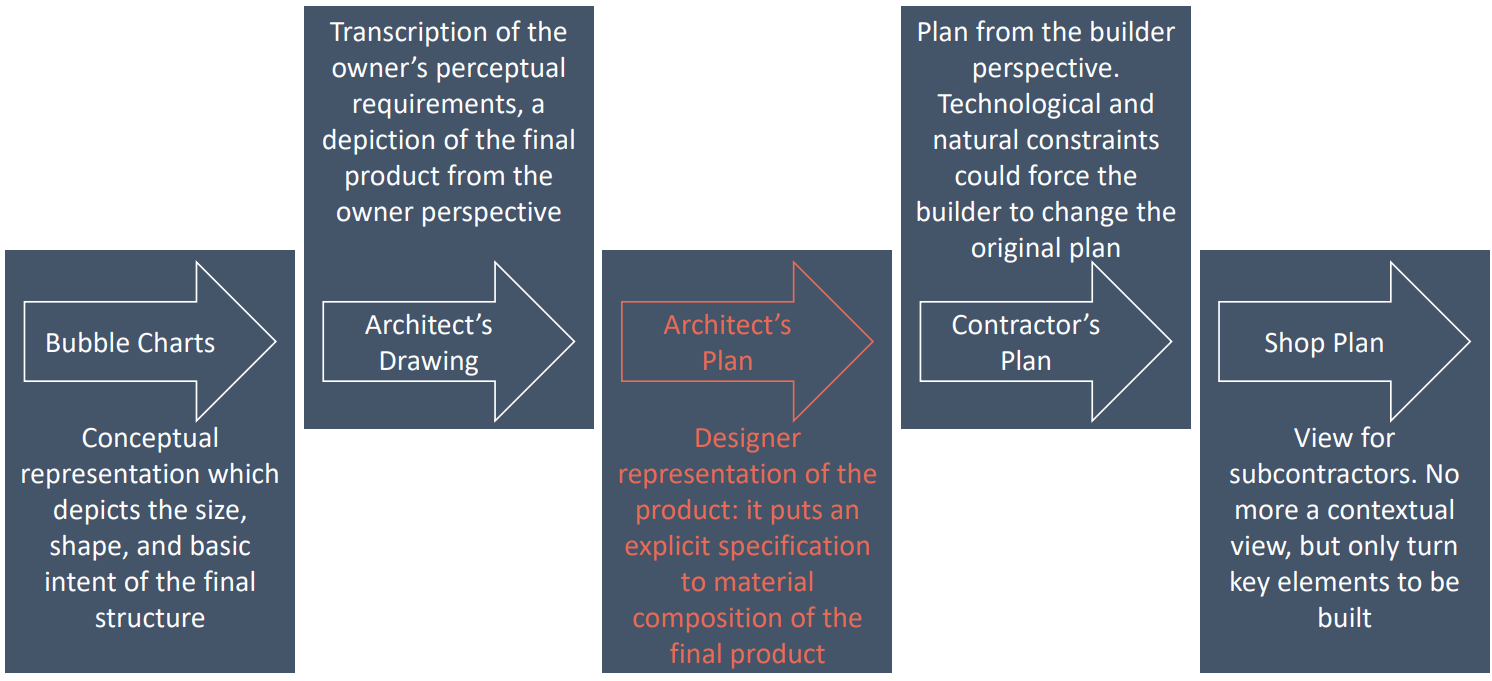
\includegraphics[scale=0.3]{1-zachman-framework-for-building}
\end{center}

\subsubsection{Zachman Framework for Information System}
\begin{center}
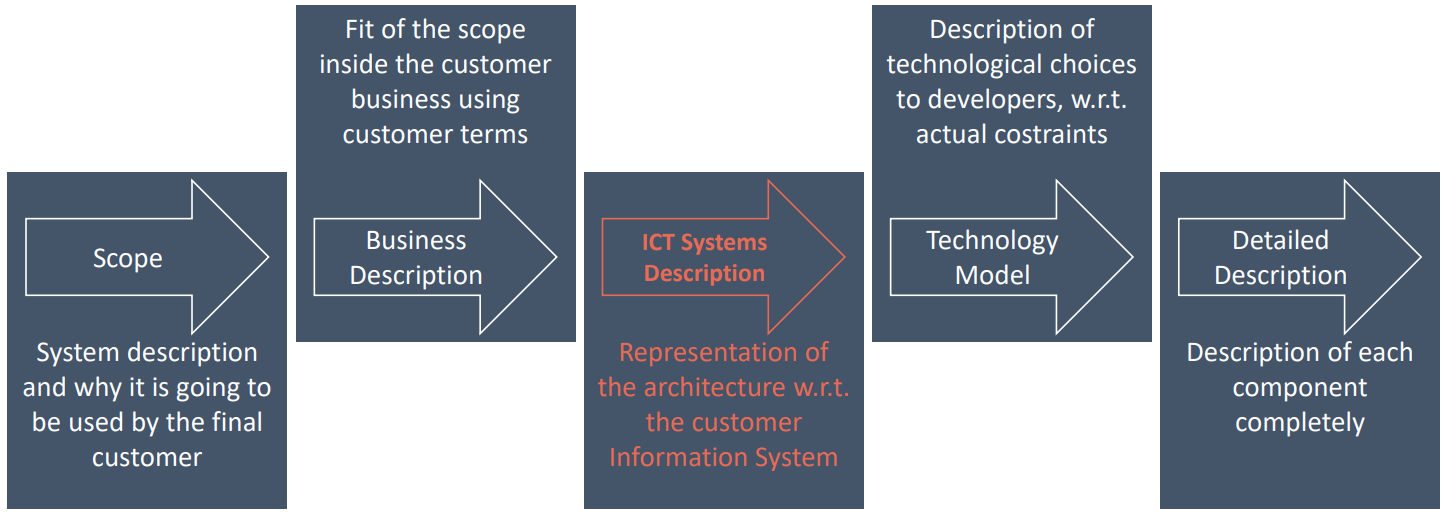
\includegraphics[scale=0.3]{2-zachman-framework-for-information-system}
\end{center}

\subsubsection{Different point of views}
Each perspective is not just a matter of different level of detail.

It is linked with \textbf{different natures} and \textbf{accountability}.

\begin{itemize}
	\item \textbf{Input-Process-Output}
	
	Product description in detail w.r.t. intended capabilities, appearance, and interactions with users
	
	\item \textbf{Entity-Relationship-Entity}
	
	<<Stuff things is made of>>, description of data in each building blocks
	
	\item \textbf{Node-Line-Node}
	
	Flows between each component
\end{itemize}

\subsection{Architectural Styles}

\textbf{Software Architecture}
A software architecture is a set of \textbf{architectural elements} that have a particular form.
\begin{center}
[...]
\end{center}
The architectural form consists of weighted \textbf{properties} and \textbf{relationship}.
\begin{center}
[...]
\end{center}
An underlying, but integral, part of an architecture is the rationale for the various choice made in defining an architecture.

\subsubsection{Building Architecture}
\textbf{Building Architecture exploits different ARCHITECTURAL STYLES}

\textbf{Descriptively}, architectural style defines a particular codification of \textbf{design elements} and formal arrangements.

\textbf{Prescriptively}, style limits the kinds of design elemetns and their \textbf{formal arragements}.

That is, an architectural style constrains both the \textbf{design elements} and the \textbf{formal relationship} among the degign elements.

\subsubsection{\sout{Building} Software Architecture}

\textbf{\sout{Building} Software Architecture exploits different ARCHITECTURAL STYLES}

Architectural Style \textbf{encapsulates} important decision about elements and emphasizes important constraints on them and their relationships. 

We can use Architecture Style both to \textbf{constrain} the architecture and to \textbf{coordinate} cooperating architects.

Moreover, style \textbf{embodies} those decision that suffer \textbf{erosion and drift}: an emphasis on it as a constraint on the architecture provides a visibility to certain aspects of the architecture so that violations of those aspects and insesnsitivity of them will be more obvious.

\subsubsection{Elements}

\begin{center}
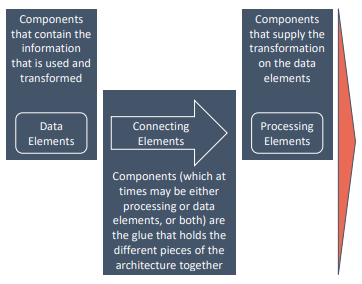
\includegraphics[scale=0.7]{3-architectural-styles-elements}
\end{center}

\textbf{Properties} are used \textbf{to constrain the choice of architectural elements}. They define the minimum desired constraints unless otherwise stated: by default on "what is not constrained by the architect may take any form desired by the designer or implementer"

\textbf{Relationship} are used \textbf{to constrain the "placement" of architectural element} - how the different elements may interact and how they are organized with respect to each other in the architecture

\textbf{Rationale} is an underlying. but integral, part of an architecture for the various choices mad in defining an acrchitexture. \textbf{It captures the motivation for the choice of architectural style, the choice of elements, and the form to satisfy the system constraints}

\subsubsection{Enterprise Architecture Styles}

\begin{enumerate}
	\item \textbf{\textit{1990 - Common Object Request Broker Architecture - COBRA}}
	\textit{"Framework to allow objects hosted in different systems to make remote procedures call via a computer network using an Object Request Broker which marshals and serializes these requests"}	
	
	\item \textbf{\textit{2003 - Service Oriented Architecture - SOA}}
	\textit{"Framework for integrating business processes and supporting IT infrastructure as secure, standardized components - services - that can be reused and combined to address changing business priorities"} Bieberstein, Bose et al. 2005
	
	1. 2012 - Microservices
	
	\item \textbf{\textit{2004 - Message Oriented Architecture - MOM}}
	"Framework to allow objects hosted in different systems to send messages via a computer network using Message Broker to distribuite Application modules over heterogeneous platform"

	\item ...	
\end{enumerate}

\subsection{Style and Material}

\subsubsection{Building Architecture}

\textbf{Classical Architecture combines STYLE and MATERIALS}

The materials have \textbf{certain properties} that are exploited in providing a particular style. One may combine structural with aesthetic uses of materials, such as that found in the post and beam construction of tudor-style houses.

However, \textbf{one does not build a skyscraper with wooden posts} and beams.

The \textbf{material aspects} of the design elements provide both aesthetic and engineering bases for an architecture.

\subsubsection{\sout{Building} Software Architecture}

\textbf{\sout{Building} Software Architecture combines STYLE and MATERIALS}

The same function can be obtained using \textbf{different subsystems}.

To train a \textbf{Neural Network Python} could be the best fit, while to put the trained Network in production using \textbf{FPGA} to physically build the network could be a better solution.

\subsection{When an Architecture is designed}
\begin{center}
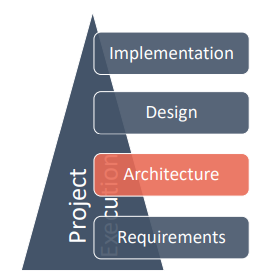
\includegraphics[scale=0.7]{4-when-an-architecture-is-designed}
\end{center}

\begin{itemize}
	\item Implementation: Representations of the algorithms and data types that satisfy the \textbf{design, architecture} and \textbf{requirements}
	
	\item Design: Modularization and detailed interfaces of the design elements, their algorithms and procedures, and the data types needed to support the \textbf{architecture} and to satisfy the requirements.
	
	\item Architecture: Selection of \textbf{architectural elements}, thier \textbf{interactions}, and the \textbf{constraints} to provide a framework in which to satisfy the \textbf{requirements} and serve as a basis for the \textbf{design}
	
	\item Requirements: Determination of the information, processing, and the characteristics of that information and processing needed by the user of the system
\end{itemize}

There new problems involve the system-level design of software, in which the important decisions are concerned with the kinds of modules and subsystems to use and the may these modules and subsystems are organized.

This level of organization, the software architecutre level, requires new kinds of abstractions that capture essential properties of major subsystems and the ways thay interact.

\subsection{Architecture as a framework for abstractions}
\begin{itemize}
	\item The essence of \textbf{abstraction} is recognizing a pattern, naming and defining it, analyzing it, inding ways to specify it, and providing some way to invoke the pattern by its name without error-prone manual intervention
	\item This process \textbf{suppresses the detail of the pattern's implementation}, reduces the opportunity for clerical error, and simplifies understanding of the result
	\item In other words, good abstraction is \textbf{ignoring the right detail} at the right times
\end{itemize}

\textit{"The development of \textbf{individual abstractions} often follows a common pattern:}
\begin{itemize}
	\item \textit{First, problems are \textbf{solved ad hoc}}
	\item \textit{As experience accumulates, some solutions turn out to work better than others, and \textbf{a sort of solklore is passed informally} from person to person}
	\item \textit{Eventually the useful solutions are understood more systematically, and they are \textbf{codified} and analyzed}
	\item \textit{This in turn enables \textbf{a more sphisticated level of} practice and allows us to tackle harder problems"}
\end{itemize}

\subsubsection{Example of Abstraction}

\begin{center}

\textbf{First example}

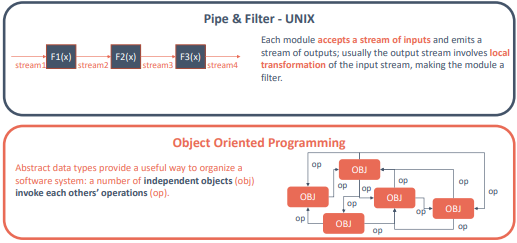
\includegraphics[scale=0.7]{5-example-of-abstraction}

\textbf{Second example}

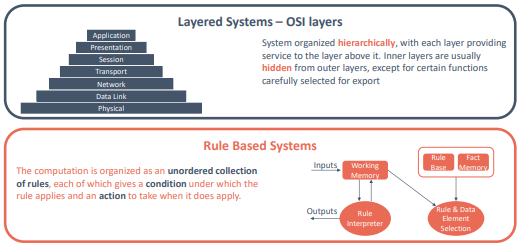
\includegraphics[scale=0.7]{6-example-of-abstraction}
\end{center}

\subsubsection{System-subsystem Abstraction}

System are constructed by combining \textbf{subsystems}:
\begin{itemize}
	\item indipendently \textbf{compilable modules}, linked by shared data or procedure calls
	\item sets of \textbf{design decisions} and the \textbf{code} that implements them
	
Subsystem \textbf{have an internal structure}. It is often useful to design that substructure at an architectural level before implementing it
\end{itemize}

Each subsystem may performs:
\begin{itemize}
	\item a \textbf{specific function} to the system begin implemented
	\item a \textbf{more common function} such as communication or storage
\end{itemize}

\textbf{Identifying} and \textbf{classifying} the system functions that are common to many applications is a significant first step to the development of a software architecture.

\subsection{BOC-App}

\subsubsection{Bully Operation Center}
A WebApp supports a \textbf{group of Analysts} to spot \textbf{aggressive users}. 

Natural Language Processing is used to \textbf{classify} each tweets.

When the \textbf{number of aggressive tweets} done by a given user go beyond a given threshold, this user is surfaced to an Analyst \textbf{who can decide to ban} it.

When a user is classified by the Analyst as bully, \textbf{the number of bullied users} iscomputed as the number of users after a bully user comment stop to use tweeter.

\subsubsection{Problem Abstraction}
\begin{center}
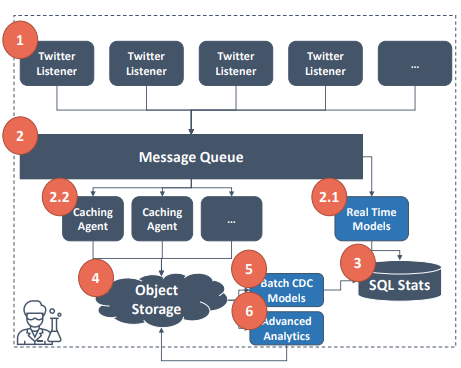
\includegraphics[scale=0.7]{7-boc-app-problem-abstraction}
\end{center}

\begin{enumerate}
	\item Different \textbf{Twitter Listeners} ensure:
	\begin{enumerate}
		\item \textbf{Scalability}: we can follow as many as hashtag we need
		\item \textbf{Reliability}: we can re-distribute hashtegs to other node if a given Listener fail
	\end{enumerate}
	\item A \textbf{Message Queue} allow serveral concurrent consumers on each hashtag
	\begin{enumerate}
		\item \textbf{Real Time Consumer}
		\item \textbf{Caching Consumer}
	\end{enumerate}
	\item Data \textbf{-as-is-} is saved using the \textbf{Object Storage} model for further analysis
	\item Some models \textbf{cannot be done in real time} for several reason (e.g., training a classifier)
	\item What is \textbf{I discover a given user is a bully}? I will be interested in counting a-posteriori number of users buillied by him
\end{enumerate}

\subsubsection{SubSystem Perspective}
\begin{center}
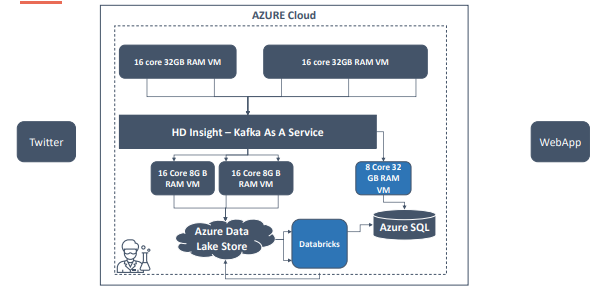
\includegraphics[scale=0.7]{8-boc-app-subsystem-perspective}
\end{center}

\subsubsection{Network Perspective}
\begin{center}
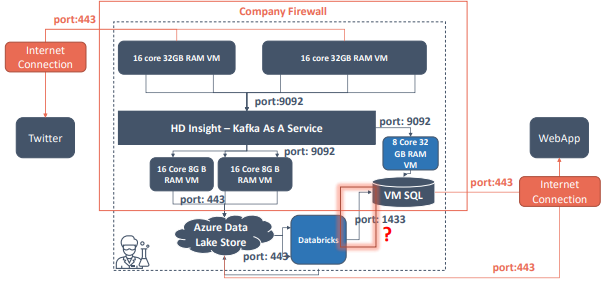
\includegraphics[scale=0.7]{9-boc-app-network-perspective}
\end{center}

\subsubsection{SQL through firewall needs care}
\begin{center}
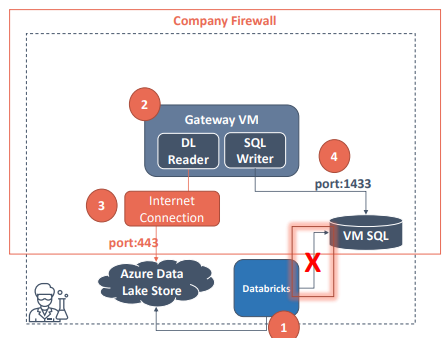
\includegraphics[scale=0.7]{10-sql-through-firewall-needs-care}
\end{center}

\begin{enumerate}
	\item Databricks writes directly on the \textbf{Data Lake}
	\item Infrastructure team create a gateway Virtual Machine in the \textbf{same network} of the SQL machine
	\item A \textbf{443 allow rule} for the Gateway is created and a Data Lake reader agent starts to read all fresh data
	\item On the same Gateway, a second agent write down data inside the SQL VM
\end{enumerate}

\subsubsection{Data Scientist Perspective}
\begin{center}
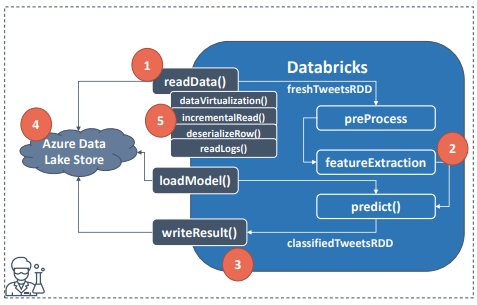
\includegraphics[scale=0.7]{11-data-scientist-perspective}
\end{center}

\begin{enumerate}
	\item Data Scientist knows using \textbf{BOCArc.readData()} will receive \textbf{e fresh tweets}
	\item Then he/she can \textbf{focus} on the code needed to clean data, extract \textbf{features} and \textbf{predict}
	\item At the end, he/she will call the \textbf{BOCArc.writeResult()} method which automagically writes result \textbf{somewhere}
	\item He/she won’t know all tweets are
written on the \textbf{Data Lake}
	\item He/she won’t know readData() hides:
	\begin{enumerate}
		\item A \textbf{virtualization layer} to decouple physical data with needed one
		\item a \textbf{CDC strategy implemented} to get only fresh tweets
		\item Tecnhical features such as \textbf{deserialization} and \textbf{log tracing}
	\end{enumerate}
\end{enumerate}

\subsubsection{CFO Perspective}
\begin{center}
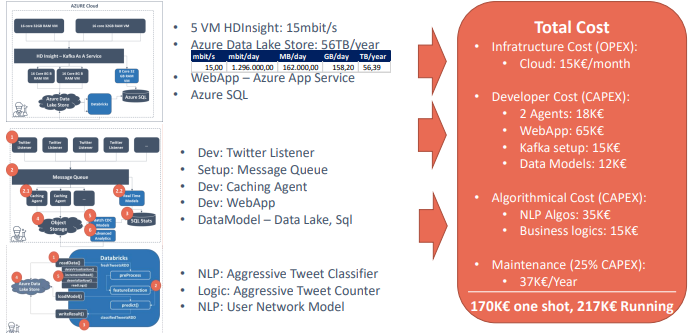
\includegraphics[scale=0.7]{12-boc-app-cfo-perspective}
\end{center}
\section{Architecture 102}

%\subsection{}

%\subsubsection{}

\textbf{Architectures:}
\begin{itemize}
	\item The art or practice of \textbf{designing} and \textbf{building} structure and especially habitable ones.
	\item A unifying or coherent \textbf{from} or \textbf{structure}
\end{itemize}

\textbf{Foundation for the study of Software Architecture / L. Wolf, 1992}

Software architecure principles can be \textbf{inherited} by appealing to several well-established architectural disciplines.

While the subject matter for the two is quite different, there are a number of intresting \textbf{architectural points} in building architecture that are suggestive for software architecture
\begin{itemize}
	\item multimple \textbf{views}
	\item architectural \textbf{styles}
	item style and \textbf{materials}
+\end{itemize}

\subsection{Preliminary Concept}

\textbf{Never take anything for granted}

\subsubsection{Apache Kafka and Pub/Sub}

\begin{itemize}
	\item Kafka is a \textbf{distributed system} consisting of servers and clients that communicate via a high-performance TCP network protocol.
	\item Kafka combines three key capabilities so tou can implement your use cases for \textbf{event streaming end-to-end}
	\begin{itemize}
		\item To \textbf{To publish (write} and \textbf{subscribe to} (read) streams of events, including continuous import/export of your data from other system
		\item To \textbf{store} streams of events durably and reliably for as long as you want
		\item To \textbf{process} streams of events as they occur or retrospectively
	\end{itemize}
	\item An \textbf{event} records the fact that "something happened" in the world or in your business [e.g., a user posts a tweet]
	\item \textbf{Producers} are those client applications that publish (write) events to Kafka, and \textbf{consumers} are those that subscribe to (read and process) these events. In Kafka, \textbf{producers and consumers are fully decoupled and agnostic of each other}, which is a key design element to achieve the high scalability that Kafka is known for.
	\item Events are organized and durably stored in \textbf{topics}. Very simplified, a topic is similar to a folder in a filesystem, and the events are the files in that folder. Another way to see it, the \textbf{topic is like an INDEX} on a SQL table.
\end{itemize}

\subsubsection{Extract Transform Load – ETL (*)}

\begin{itemize}
	\item In computing, extract, transform, load (ETL) is the general procedure of \textbf{copying data from one or more sources into a destination system}
	\begin{itemize}
		\item Data extraction involves \textbf{extracting data from homogeneous or heterogeneous} sources
		\item Data transformation processes data by \textbf{data cleaning and transforming them into a proper storage format/structure} for the purposes of querying and analysis
		\item Data loading describes \textbf{the insertion of data into the final target database} such as an operational data store, a data mart, data lake or a data warehouse
	\end{itemize}
	\item ETL can be used:
	\begin{itemize}
		\item to increase data quality and consistency
		\item to normalize data
		\item to apply simple/complex logics such as id to string conversion through a lookup table
		\item to prepare data for a presentation layer
	\end{itemize}
	\item ETL can be one-shot or incremental
\end{itemize}

\subsubsection{Object Storage Model}
\begin{itemize}
	\item Object storage is a \textbf{computer data storage architecture} that manages data asobjects. It is opposed to other storage architectures like file systems or block storage
	\item Each object typically contains \textbf{data, contextual information} (metadata), and \textbf{technical information} (header)
	\item It is based on a \textbf{shared naming convention}, which generates a unique id for each object, and a shared \textbf{serialization strategy} (e.g., json)
	\item It allows to \textbf{distribute data} over several nodes
	\item Object storage was created to allow \textbf{retention} of massive amounts of unstructured data
\end{itemize}

\subsubsection{Data Lake}
\begin{itemize}
	\item Models you can build using data cannot \textbf{be known a priori}: if some pieces ofinformation are not saved when produced (e.g., under sampling a sensor), they \textbf{could not be re-acquired later}
	\item \textbf{Legacy Systems} integration is pretty complex and expensive: once a legacy system is integrated, there is no reason not to get all available information
	\item Other Data Architectures have problems dealing with \textbf{heterogeneous data} or data which format and content can \textbf{change over time}
	\item Data Lakes is based on \textbf{four pillars}:
	\begin{itemize}
		\item Unprocessed data (only serialized in objects)
		\item Data saved forever
		\item Good reading/writing performances
		\item Schema available on read
	\end{itemize}
\end{itemize}

\subsubsection{Concrete and Abstract Classes}
\begin{itemize}
	\item Concrete Class
	\begin{itemize}
		\item A concrete class is a class that can be instantiated
	\end{itemize}
	\item Abstract Class
	\begin{itemize}
		\item Cannot be instatied
		\item Contains Abstract Methods
		\item Can contain concrete methods
		\item Specifies virual methods via signatures that are to be implemented
		\item Before a class derived from an abstract class can be instantiated, all abstract methods of its parent classes must be implemented
	\end{itemize}
\end{itemize}

\subsubsection{Lock-in}
\begin{itemize}
	\item Vendor lock-in makes \textbf{a customer dependent on a vendor} for products and
services
	\item A supplier \textbf{successfully locks in} a customer when:
	\begin{itemize}
		\item \textbf{the cost of changing} supplier is higher that the cost of keeping it
		\item without that cost, other \textbf{suppliers can outperform} the actual supplier
	\end{itemize}
	\item An Enterprise Architecture can protect the company from Vendor lock-in
	\item Another kind of lock-in is the so called \textbf{knowledge lock-in}: this kind of lock-in happens when the \textbf{cost of knowledge transfer} is higher than the benefit to dismiss a person/team. Again, a Software Architecture can \textbf{mitigate this risk}
\end{itemize}

\subsection{Software Architecture Pillars}

\subsubsection{8 reasons why}

\begin{center}
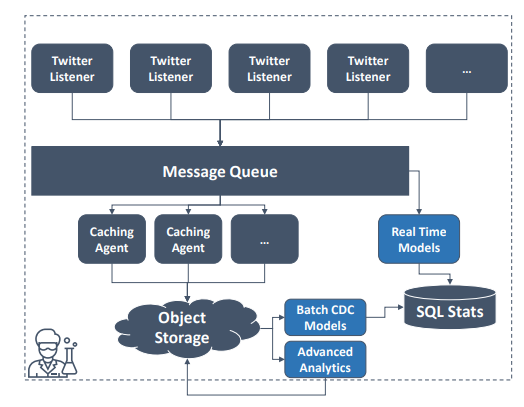
\includegraphics[scale=0.7]{13-architecture-pillars-on-BOC-app}
\end{center}

\textbf{Bully Operation Center}
\begin{itemize}
	\item A WebApp supports \textbf{a group of Analysts} to spot \textbf{aggressive users}
	\item Natural Language Processing is used to \textbf{classify} each tweets
	\item When the \textbf{number of aggressive tweets} done by a given user go beyond a given threshold, this user is surfaced to an Analyst \textbf{who can decide to ban} it
	\item When a user is classified by the Analyst as bully, \textbf{the number of mbullied users} is computed as the number of users after a bully user comment stop to use tweeter
\end{itemize}

\subsubsection{Software Architecture Pillars}
\begin{enumerate}
	\item Being the framework for satisfying requirements
	\item Being the technical basis for design 
	\item Being the managerial basis for cost estimation and process management
	\item Enabling component reuse
	\item Focus on centralization
	\item Enhancing productivity and security
	\item Enabling enterprise systems integration (Enterprise Application Integration)
	\item Allowing a tidy scalability
	\item Controlling software processes execution
	\item Avoiding handover and people lock-in
\end{enumerate}

\subsubsection{Being the framework for satisfying requirements}
\begin{center}
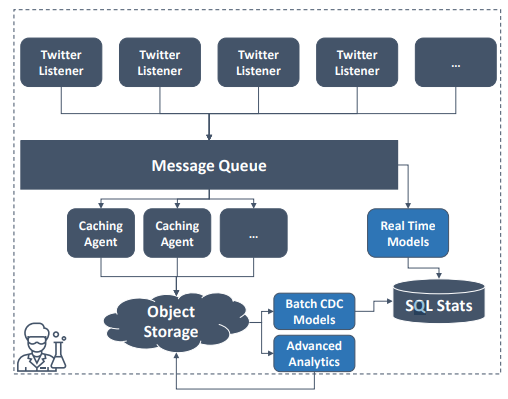
\includegraphics[scale=0.7]{14-being-the-framework-for-satisfying-requirements}
\end{center}
\begin{itemize}
	\item Functional Requirement
	\begin{itemize}
		\item Am I able to spot aggressive users?
		\item Will the Analyst have all the needed information to decide to ban a user?

	\end{itemize}
	\item Technical Requirement
	\begin{itemize}
		\item Am I able to process all the tweets in time?
		\item Am I able to check in the history bullied users?
	\end{itemize}
	\item Security Requirement
	\begin{itemize}
		\item Is it compliance with GDPR (data privacy rules)?
	\end{itemize}
\end{itemize}

\subsubsection{Being the technical basis for design}
\begin{center}
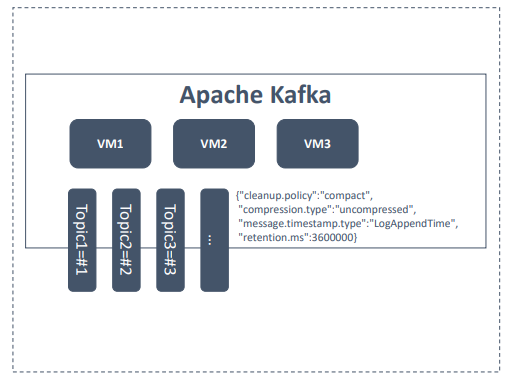
\includegraphics[scale=0.5]{15-being-the-technical-basis-for-design}
\end{center}

Modularization and detailed interfaces of the design elements, their algorithms and procedures, and the data types needed to support the architecture and to satisfy the requirements

\subsubsection{Being the managerial basis for cost estimation and process
management}
\begin{center}
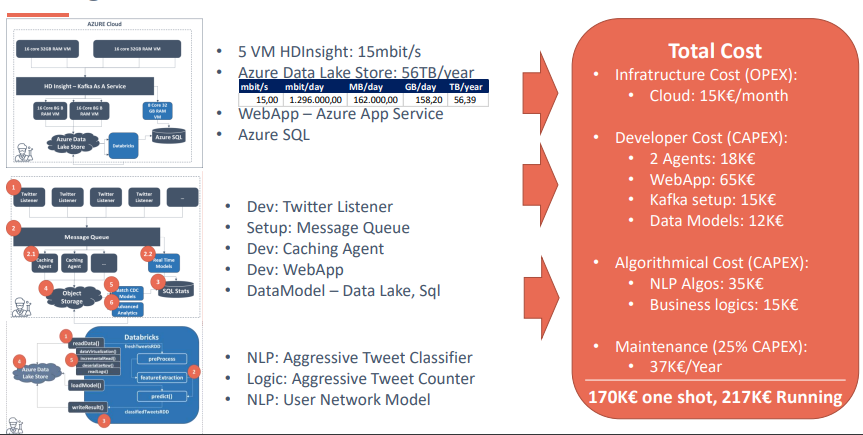
\includegraphics[scale=0.5]{16-being-the-managerial-basis-for-cost-estimation-and-process}
\end{center}

\subsubsection{Enabling component reuse}
\begin{center}
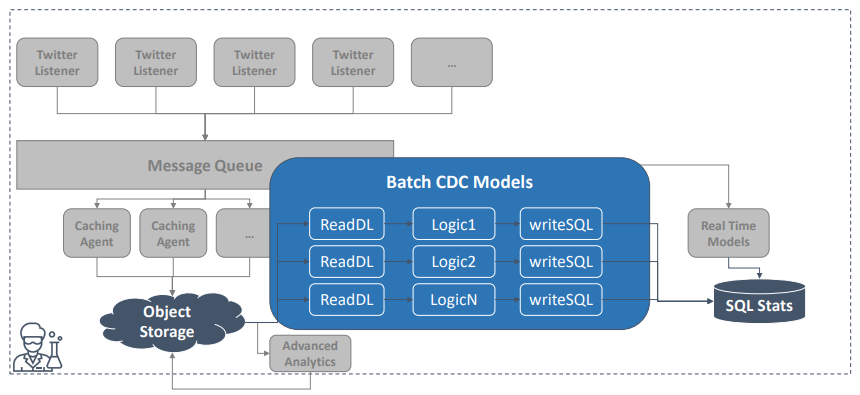
\includegraphics[scale=0.5]{17-enabling-component-reuse}
\end{center}

\subsubsection{Focus on centralization}
\begin{center}
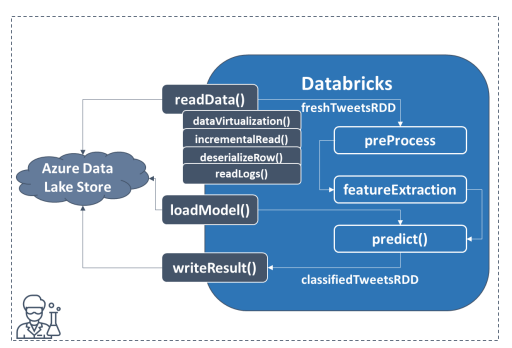
\includegraphics[scale=0.7]{18-focus-on-centralization}
\end{center}

\begin{itemize}
	\item Azure Data Lake Store in our Architecture is the Single Source of Truth
	\item Data are Centralized there
\end{itemize}

\subsubsection{Enhancing productivity and security}
\begin{center}
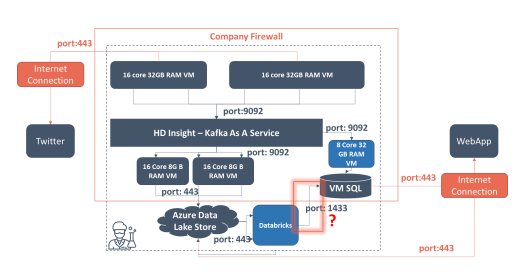
\includegraphics[scale=0.9]{19-enhancing-productivity-and-security}
\end{center}

\begin{itemize}
	\item We know exactly which ports we need to open
	\item We can build a gateway to access SQL data from WebApp to avoid SQL Injection (access is centralized there)
	\item We can build the component to hide Data Lake and enforce ACL Rules
\end{itemize}

\subsection{Design patterns}
\textbf{are formalized best practices found to solve common problems}

\subsubsection{Hundreds of Design Pattern}
\begin{center}
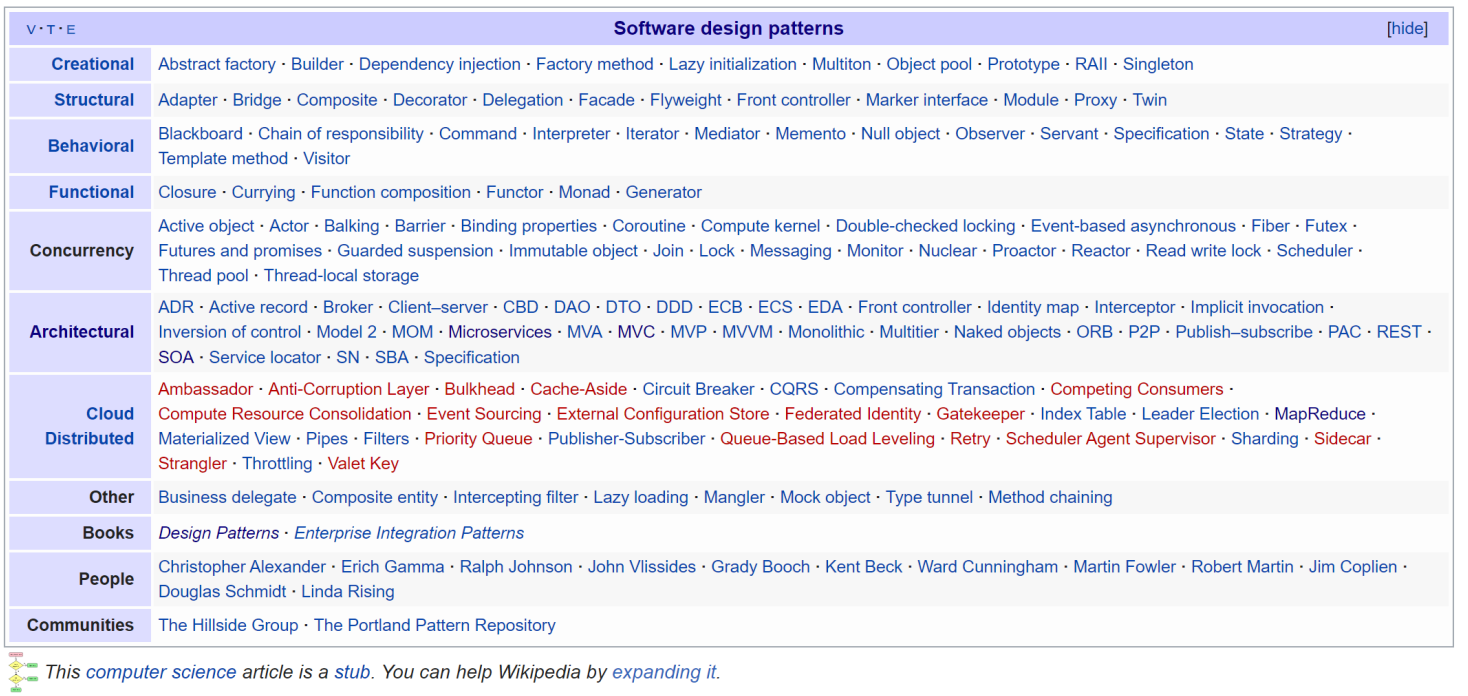
\includegraphics[scale=0.35]{20-hundreds-of-degisn-pattern}
\end{center}

\subsubsection{The 23 Classical Patterns by Type}
\begin{center}
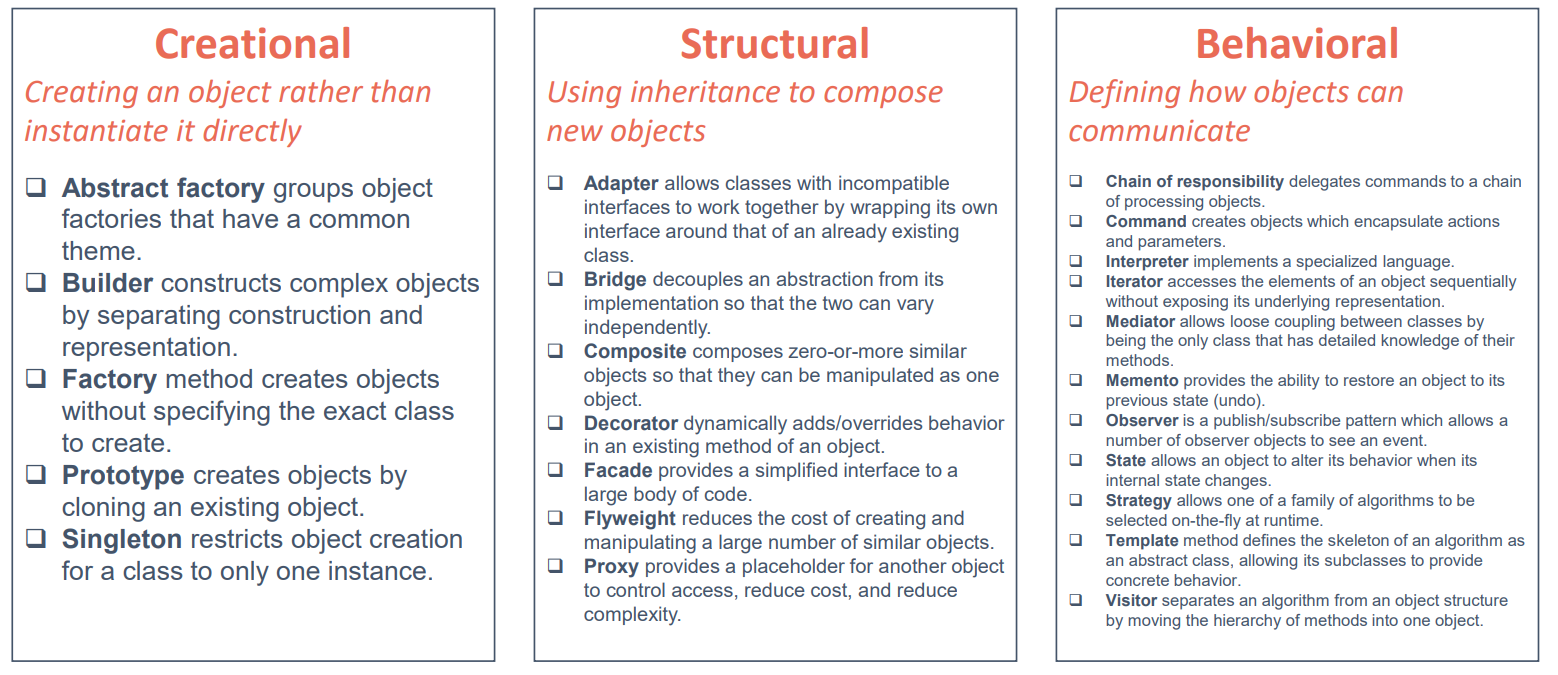
\includegraphics[scale=0.3]{21-the-23-classical-pattern-by-type}
\end{center}

\subsubsection{A classic Big Data challenge}
\begin{center}
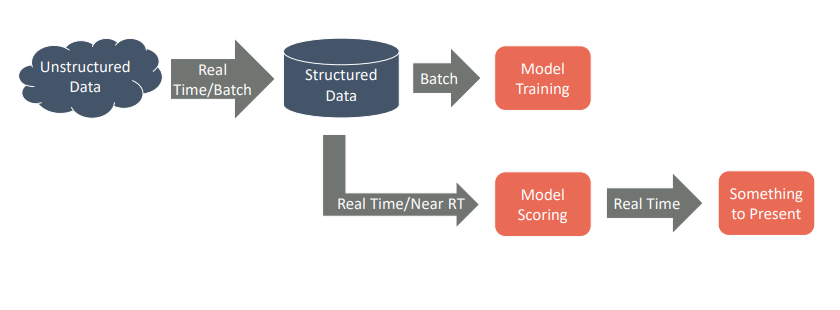
\includegraphics[scale=0.3]{22-a-claassic-big-data-challenge}
\end{center}

\subsubsection{From ETL to ELT}
\begin{center}
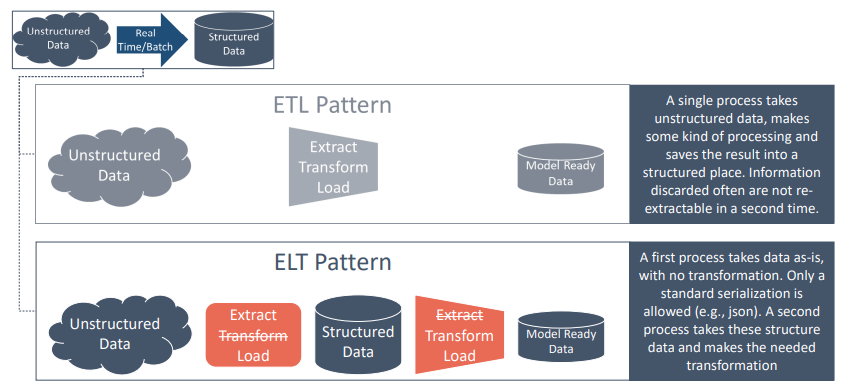
\includegraphics[scale=0.3]{23-from-etl-to-elt}
\end{center}
\section{Architecture 103}

\subsection{Preliminary concept}

\textbf{State - Stateful - Stateless}

\begin{itemize}
	\item State
	variable and instances of a system at a given time
	\item Stateful
	capability of a system to remember preceding event or user insteraction
	e.g., an applicative session of an authenticated user on a Web Site
	\item Stateless
	capability of a system to response always in the same way independently to any sort of previus state
	e.g., a REST API
\end{itemize}

\textbf{Table index*}

\begin{itemize}
	\item An index is an optional structure, associated with a table or table cluster, that sometimes speed data access
	\item By creating an index on one or more caloumns of a table, you gian the ability in some cases to retrive a small set of randomly distributed rows from the table
\end{itemize}



\textbf{Foundation for the study of Software Architecture / L. Wolf, 1992}

Software architecure principles can be \textbf{inherited} by appealing to several well-established architectural disciplines.

While the subject matter for the two is quite different, there are a number of intresting \textbf{architectural points} in building architecture that are suggestive for software architecture
\begin{itemize}
	\item multimple \textbf{views}
	\item architectural \textbf{styles}
	item style and \textbf{materials}
+\end{itemize}

\subsection{Preliminary Concept}

\textbf{Never take anything for granted}

\subsubsection{Apache Kafka and Pub/Sub}

\begin{itemize}
	\item Kafka is a \textbf{distributed system} consisting of servers and clients that communicate via a high-performance TCP network protocol.
	\item Kafka combines three key capabilities so tou can implement your use cases for \textbf{event streaming end-to-end}
	\begin{itemize}
		\item To \textbf{To publish (write} and \textbf{subscribe to} (read) streams of events, including continuous import/export of your data from other system
		\item To \textbf{store} streams of events durably and reliably for as long as you want
		\item To \textbf{process} streams of events as they occur or retrospectively
	\end{itemize}
	\item An \textbf{event} records the fact that "something happened" in the world or in your business [e.g., a user posts a tweet]
	\item \textbf{Producers} are those client applications that publish (write) events to Kafka, and \textbf{consumers} are those that subscribe to (read and process) these events. In Kafka, \textbf{producers and consumers are fully decoupled and agnostic of each other}, which is a key design element to achieve the high scalability that Kafka is known for.
	\item Events are organized and durably stored in \textbf{topics}. Very simplified, a topic is similar to a folder in a filesystem, and the events are the files in that folder. Another way to see it, the \textbf{topic is like an INDEX} on a SQL table.
\end{itemize}

\subsubsection{Extract Transform Load – ETL (*)}

\begin{itemize}
	\item In computing, extract, transform, load (ETL) is the general procedure of \textbf{copying data from one or more sources into a destination system}
	\begin{itemize}
		\item Data extraction involves \textbf{extracting data from homogeneous or heterogeneous} sources
		\item Data transformation processes data by \textbf{data cleaning and transforming them into a proper storage format/structure} for the purposes of querying and analysis
		\item Data loading describes \textbf{the insertion of data into the final target database} such as an operational data store, a data mart, data lake or a data warehouse
	\end{itemize}
	\item ETL can be used:
	\begin{itemize}
		\item to increase data quality and consistency
		\item to normalize data
		\item to apply simple/complex logics such as id to string conversion through a lookup table
		\item to prepare data for a presentation layer
	\end{itemize}
	\item ETL can be one-shot or incremental
\end{itemize}

\subsubsection{Object Storage Model}
\begin{itemize}
	\item Object storage is a \textbf{computer data storage architecture} that manages data asobjects. It is opposed to other storage architectures like file systems or block storage
	\item Each object typically contains \textbf{data, contextual information} (metadata), and \textbf{technical information} (header)
	\item It is based on a \textbf{shared naming convention}, which generates a unique id for each object, and a shared \textbf{serialization strategy} (e.g., json)
	\item It allows to \textbf{distribute data} over several nodes
	\item Object storage was created to allow \textbf{retention} of massive amounts of unstructured data
\end{itemize}

\subsubsection{Data Lake}
\begin{itemize}
	\item Models you can build using data cannot \textbf{be known a priori}: if some pieces ofinformation are not saved when produced (e.g., under sampling a sensor), they \textbf{could not be re-acquired later}
	\item \textbf{Legacy Systems} integration is pretty complex and expensive: once a legacy system is integrated, there is no reason not to get all available information
	\item Other Data Architectures have problems dealing with \textbf{heterogeneous data} or data which format and content can \textbf{change over time}
	\item Data Lakes is based on \textbf{four pillars}:
	\begin{itemize}
		\item Unprocessed data (only serialized in objects)
		\item Data saved forever
		\item Good reading/writing performances
		\item Schema available on read
	\end{itemize}
\end{itemize}

\subsubsection{Concrete and Abstract Classes}
\begin{itemize}
	\item Concrete Class
	\begin{itemize}
		\item A concrete class is a class that can be instantiated
	\end{itemize}
	\item Abstract Class
	\begin{itemize}
		\item Cannot be instatied
		\item Contains Abstract Methods
		\item Can contain concrete methods
		\item Specifies virual methods via signatures that are to be implemented
		\item Before a class derived from an abstract class can be instantiated, all abstract methods of its parent classes must be implemented
	\end{itemize}
\end{itemize}

\subsubsection{Lock-in}
\begin{itemize}
	\item Vendor lock-in makes \textbf{a customer dependent on a vendor} for products and
services
	\item A supplier \textbf{successfully locks in} a customer when:
	\begin{itemize}
		\item \textbf{the cost of changing} supplier is higher that the cost of keeping it
		\item without that cost, other \textbf{suppliers can outperform} the actual supplier
	\end{itemize}
	\item An Enterprise Architecture can protect the company from Vendor lock-in
	\item Another kind of lock-in is the so called \textbf{knowledge lock-in}: this kind of lock-in happens when the \textbf{cost of knowledge transfer} is higher than the benefit to dismiss a person/team. Again, a Software Architecture can \textbf{mitigate this risk}
\end{itemize}

\subsection{Software Architecture Pillars}

\subsubsection{8 reasons why}

\begin{center}
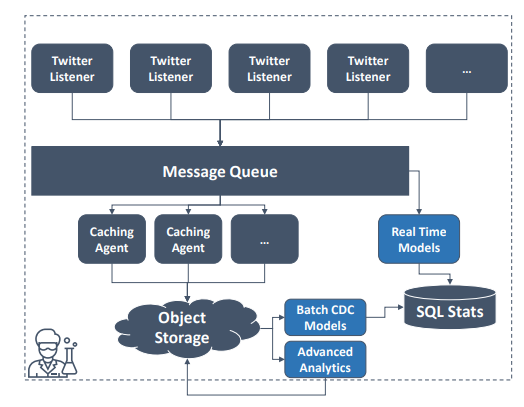
\includegraphics[scale=0.7]{13-architecture-pillars-on-BOC-app}
\end{center}

\textbf{Bully Operation Center}
\begin{itemize}
	\item A WebApp supports \textbf{a group of Analysts} to spot \textbf{aggressive users}
	\item Natural Language Processing is used to \textbf{classify} each tweets
	\item When the \textbf{number of aggressive tweets} done by a given user go beyond a given threshold, this user is surfaced to an Analyst \textbf{who can decide to ban} it
	\item When a user is classified by the Analyst as bully, \textbf{the number of mbullied users} is computed as the number of users after a bully user comment stop to use tweeter
\end{itemize}

\subsubsection{Software Architecture Pillars}
\begin{enumerate}
	\item Being the framework for satisfying requirements
	\item Being the technical basis for design 
	\item Being the managerial basis for cost estimation and process management
	\item Enabling component reuse
	\item Focus on centralization
	\item Enhancing productivity and security
	\item Enabling enterprise systems integration (Enterprise Application Integration)
	\item Allowing a tidy scalability
	\item Controlling software processes execution
	\item Avoiding handover and people lock-in
\end{enumerate}

\subsubsection{Being the framework for satisfying requirements}
\begin{center}
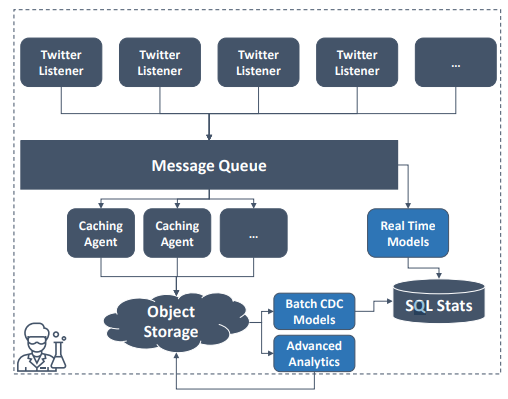
\includegraphics[scale=0.7]{14-being-the-framework-for-satisfying-requirements}
\end{center}
\begin{itemize}
	\item Functional Requirement
	\begin{itemize}
		\item Am I able to spot aggressive users?
		\item Will the Analyst have all the needed information to decide to ban a user?

	\end{itemize}
	\item Technical Requirement
	\begin{itemize}
		\item Am I able to process all the tweets in time?
		\item Am I able to check in the history bullied users?
	\end{itemize}
	\item Security Requirement
	\begin{itemize}
		\item Is it compliance with GDPR (data privacy rules)?
	\end{itemize}
\end{itemize}

\subsubsection{Being the technical basis for design}
\begin{center}
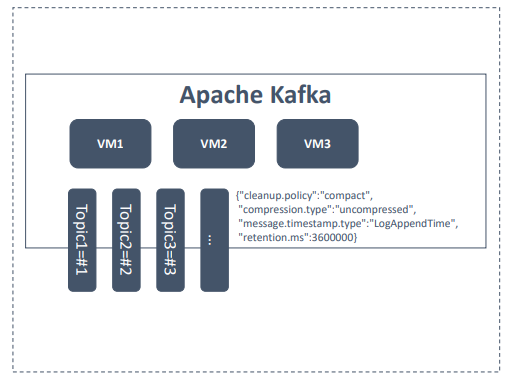
\includegraphics[scale=0.5]{15-being-the-technical-basis-for-design}
\end{center}

Modularization and detailed interfaces of the design elements, their algorithms and procedures, and the data types needed to support the architecture and to satisfy the requirements

\subsubsection{Being the managerial basis for cost estimation and process
management}
\begin{center}
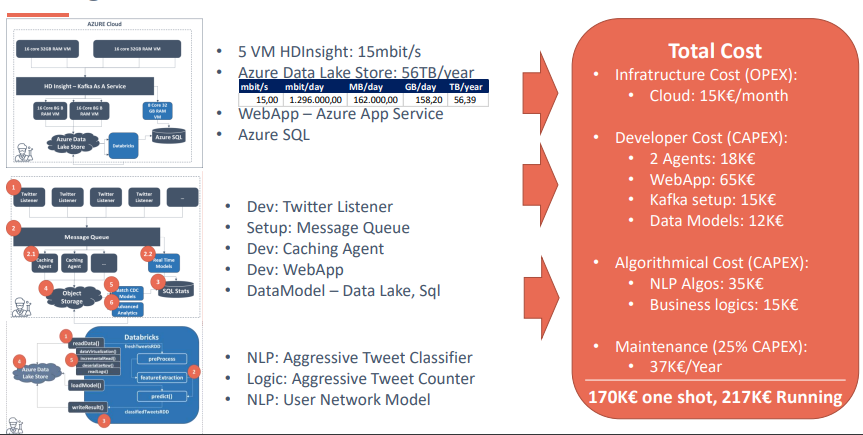
\includegraphics[scale=0.5]{16-being-the-managerial-basis-for-cost-estimation-and-process}
\end{center}

\subsubsection{Enabling component reuse}
\begin{center}
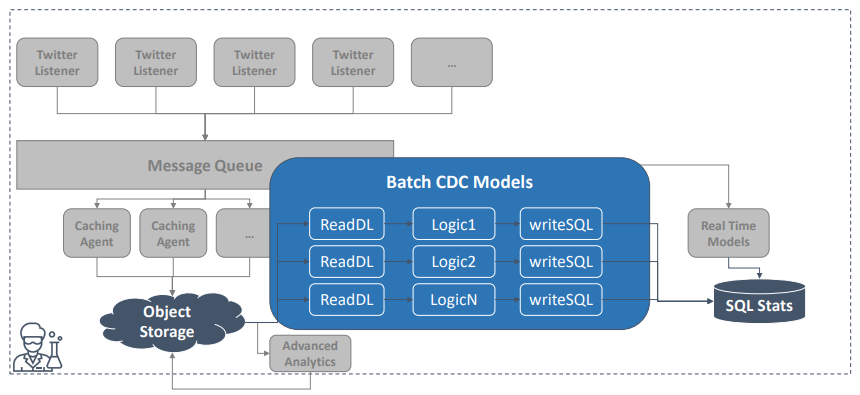
\includegraphics[scale=0.5]{17-enabling-component-reuse}
\end{center}

\subsubsection{Focus on centralization}
\begin{center}
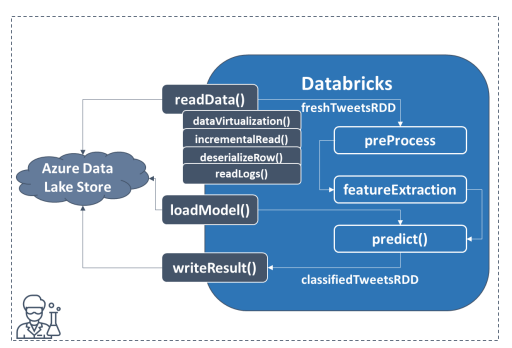
\includegraphics[scale=0.7]{18-focus-on-centralization}
\end{center}

\begin{itemize}
	\item Azure Data Lake Store in our Architecture is the Single Source of Truth
	\item Data are Centralized there
\end{itemize}

\subsubsection{Enhancing productivity and security}
\begin{center}
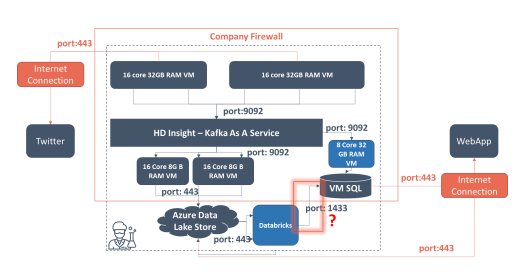
\includegraphics[scale=0.9]{19-enhancing-productivity-and-security}
\end{center}

\begin{itemize}
	\item We know exactly which ports we need to open
	\item We can build a gateway to access SQL data from WebApp to avoid SQL Injection (access is centralized there)
	\item We can build the component to hide Data Lake and enforce ACL Rules
\end{itemize}

\subsection{Design patterns}
\textbf{are formalized best practices found to solve common problems}

\subsubsection{Hundreds of Design Pattern}
\begin{center}
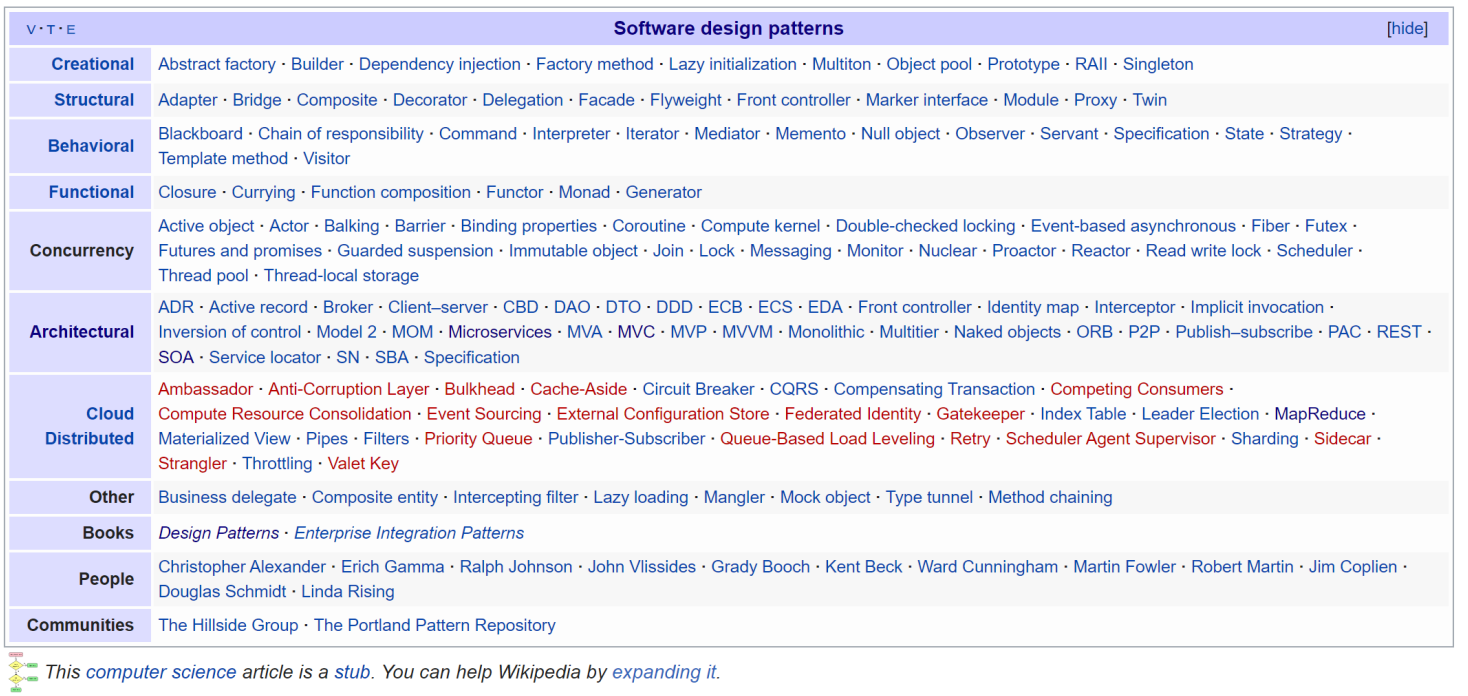
\includegraphics[scale=0.35]{20-hundreds-of-degisn-pattern}
\end{center}

\subsubsection{The 23 Classical Patterns by Type}
\begin{center}
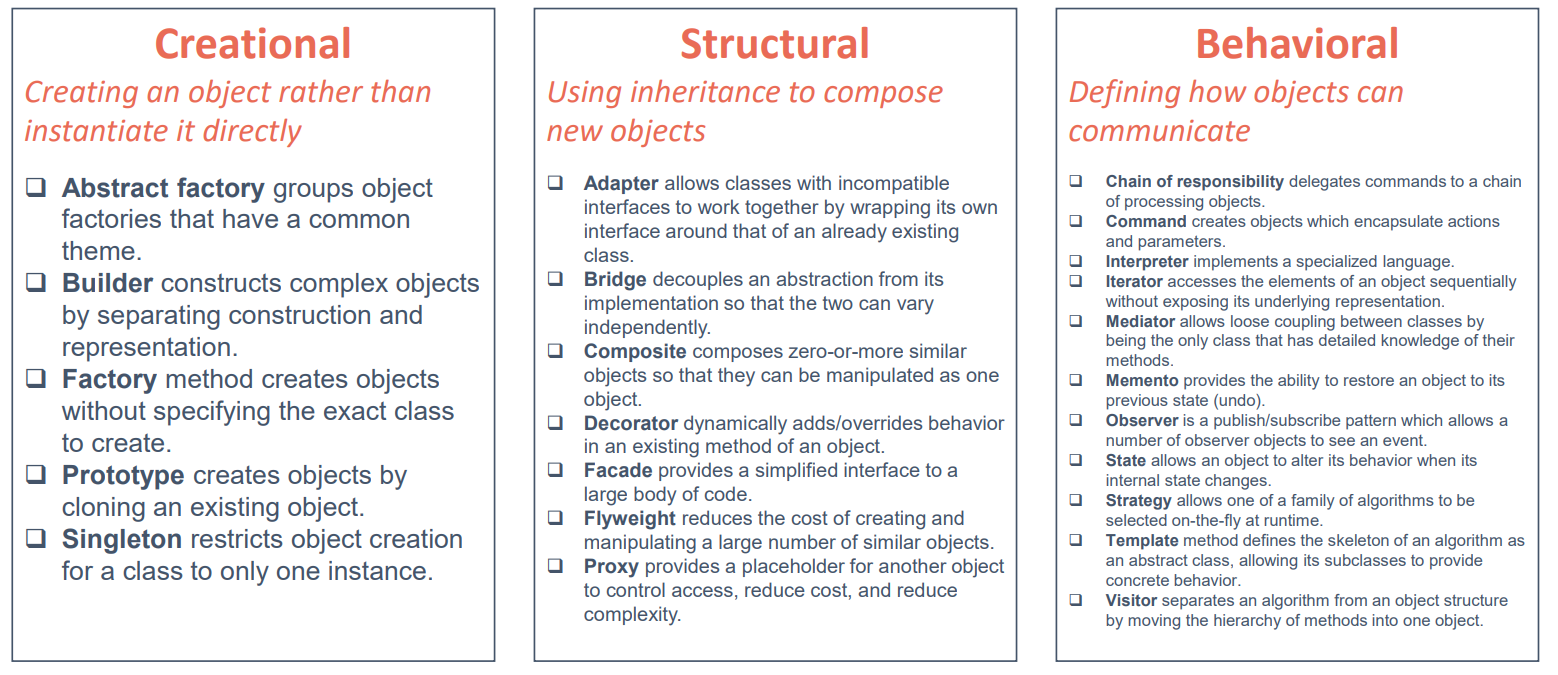
\includegraphics[scale=0.3]{21-the-23-classical-pattern-by-type}
\end{center}

\subsubsection{A classic Big Data challenge}
\begin{center}
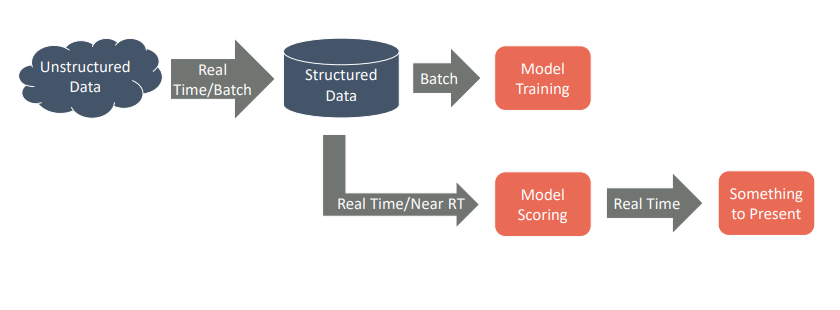
\includegraphics[scale=0.3]{22-a-claassic-big-data-challenge}
\end{center}

\subsubsection{From ETL to ELT}
\begin{center}
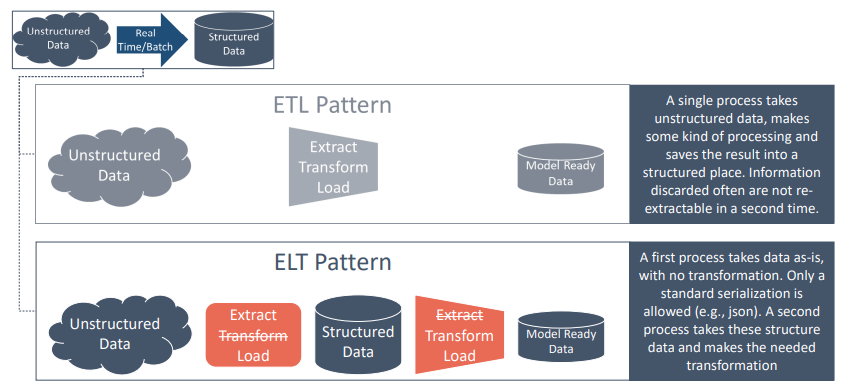
\includegraphics[scale=0.3]{23-from-etl-to-elt}
\end{center}

\section{Finally Big Data}

\subsection{Map Reduce Model}

\textbf{How can I scale the transformations to bilions of rows?}

MapReduce is a programming model proposed in a Google paper (2003)to easier multi-node process parallelization:

\begin{itemize}
	\item Users specify a map function that processes a key/value pair to generate a set of intermediate key/value pairs, and a reduce function that merges all intermediate values associated with the same intermediate key
	\item Programs written in this functional style are automatically parallelized and executed on a large cluster of commodity machines
	\item Inputs and operations over inputs are processed in parallel by different machines using a partitioning function (e.g., hash(key) mod R)
\end{itemize}  

\begin{center}
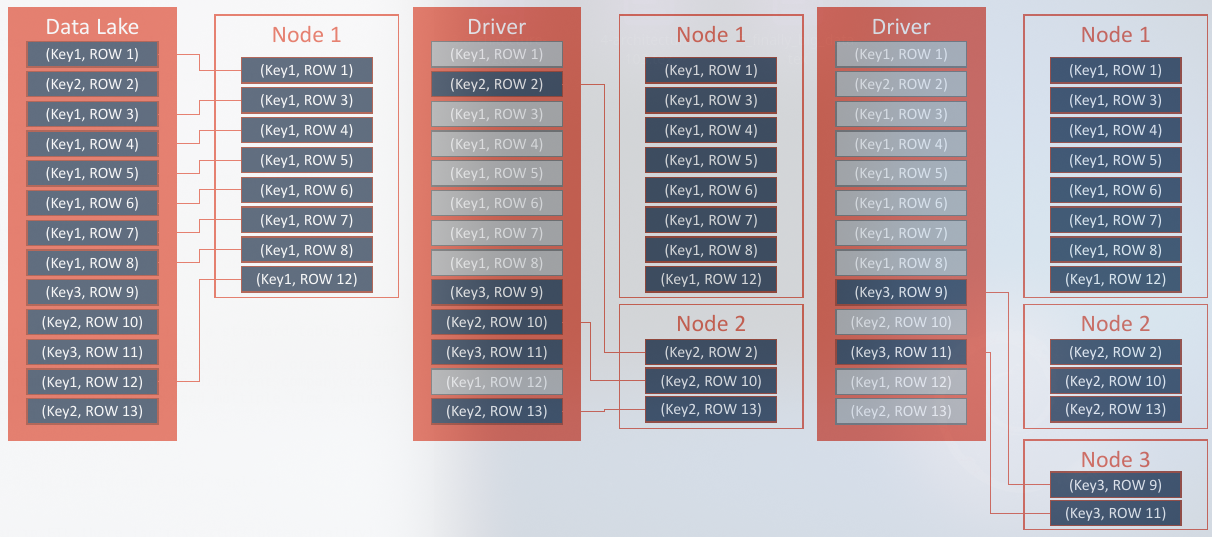
\includegraphics[scale=0.5]{51-map-reduce-model-1}
\end{center}

\begin{center}
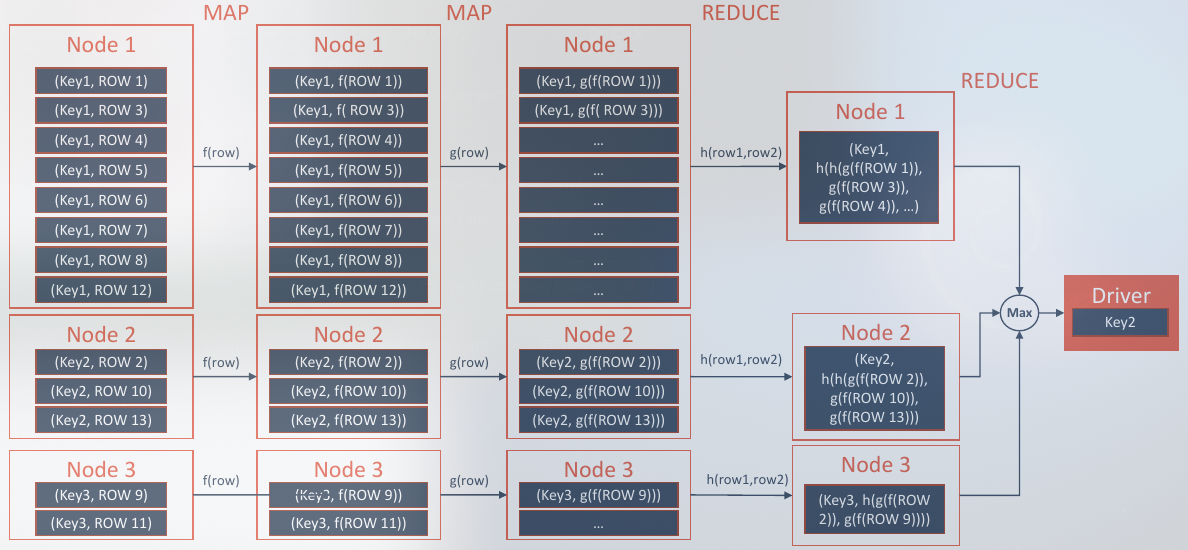
\includegraphics[scale=0.5]{51-map-reduce-model-2}
\end{center}

\subsection{Apache Hadoop}

\textbf{Distributed Parallel Frameworks}

\textbf{How to process data at scale}

\begin{itemize}
	\item Framework of -mostly- \textbf{open source components} built to facilitate the development of multi-node services written in Java
	\item Based on the assumption \textbf{hardware can fail}, several high reliability strategies are used inside Hadoop
	\item Three main components
	- \textbf{STORAGE} - Hadoop Distributed File System Storage (HDFS)
	- \textbf{RESOURCE MANAGEMENT} - Hadoop YARN
	- \textbf{PARALLEL COMPUTATION} - Hadoop MapReduce (implementation of Map Reduce pattern)
	\item Any Hadoop component should be location aware (name of the network switch where each node is) and should share it to the system to distribute data and computation
\end{itemize}

\subsection{Apache Architecture}

\begin{center}
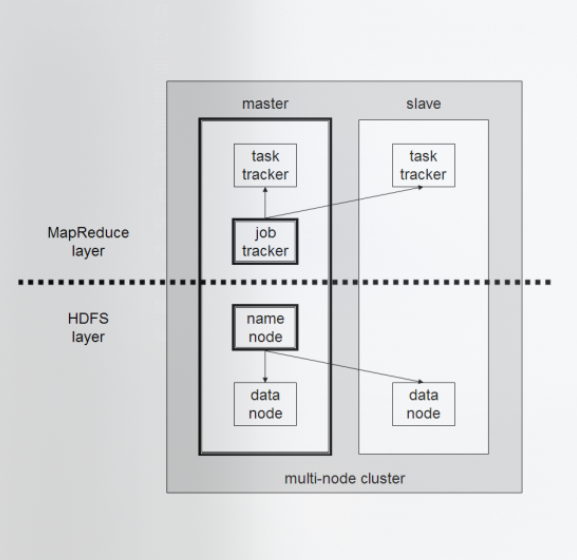
\includegraphics[scale=0.5]{52-hadoop-architecture-1}
\end{center}

\begin{itemize}
	\item \textbf{Job Tracker}
	- service that decide where a given task should be executed (ideally the nodes that have the data, or closer one)
	\item \textbf{Task Tracker}
	- a nde in the cluster that accepts tasks from a JobTracker. It expose a finite number of slots that represents its capability of run parallel tasks. Each task is executed on a spawned JVM. It also sends an heartbeat to the Job Tracker every minute to reassure it is still alive
\end{itemize}

\begin{center}
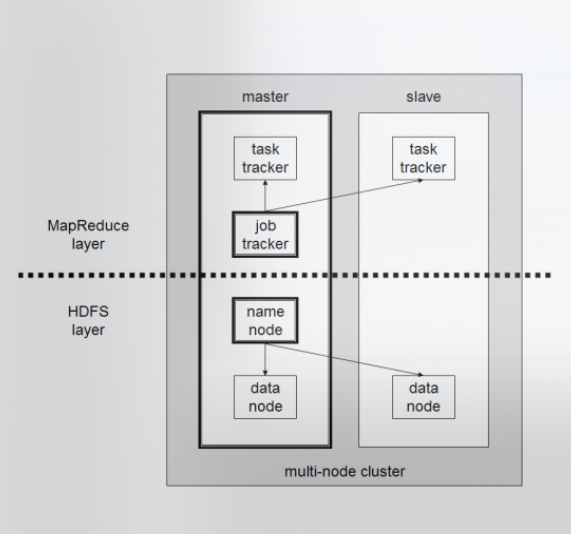
\includegraphics[scale=0.5]{52-hadoop-architecture-2}
\end{center}

\begin{itemize}
	\item \textbf{NameNode}
	- It keeps the directory tree of all files in the file system, and tracks where across the cluster the file data is kept. It does not store the data of these files itself. It is the Single Point of Failure of an Hadoop application. It routes request between application and DataNode
	\item \textbf{Backup NameNode}
	- Still under development to give to Hadoop High Availability
	\item \textbf{DataNode}
	- Stores data. DataNodes work with each other to replicate data. DataNode with data to process should be deployed on the same machine where TaskTracker is running
\end{itemize}


\end{document}
